\documentclass[a4paper,11pt]{report}

% \sloppy

%%%%%%%%%%%%%%%%%%%%%%%%%%%%%%%%%%%%%%%%%%%%%%%%%%%%%%%%%%%%
% PACKAGES
%%%%%%%%%%%%%%%%%%%%%%%%%%%%%%%%%%%%%%%%%%%%%%%%%%%%%%%%%%%%
\usepackage[utf8]{inputenc}

\usepackage[english]{babel} % francais,
\usepackage{csquotes}

\usepackage{multicol}

\usepackage{fourier}
% \usepackage{eulervm}
% NOTE: both fourier + eulervm make '<' and '>' not displaid!

\usepackage{pdflscape}

\usepackage{amsmath,amssymb,amsthm,url}
\usepackage{amsfonts}

\usepackage{subcaption}
% \usepackage{marginnote}

\usepackage{longtable}

% \usepackage[pdftex]{graphicx,color}
\usepackage[pdftex,
		colorlinks=true,
% 		pagebackref=true,
		citecolor=darkgreen,
		linkcolor=darkblue,
		urlcolor=URLCOLOR,
	]{hyperref}

\usepackage{graphicx}
\graphicspath{{./images/}{../logos/}}


% BEGIN Watermarking
\ifdefined\DraftVersion
	\usepackage{draftwatermark}
	\SetWatermarkText{draft}
	\SetWatermarkScale{2}
	\SetWatermarkColor[gray]{0.9}
\fi
% END Watermarking


\setcounter{secnumdepth}{3}

%%%%%%%%%%%%%%%%%%%%%%%%%%%%%%%%%%%%%%%%%%%%%%%%%%%%%%%%%%%%
% MARGINS, HEADERS AND FOOTERS
%%%%%%%%%%%%%%%%%%%%%%%%%%%%%%%%%%%%%%%%%%%%%%%%%%%%%%%%%%%%

\usepackage[top=1cm,bottom=2.5cm,includeheadfoot,headheight=2.5cm,\ifdefined\DraftVersion showframe \else\fi]{geometry}

% \setlength{\parskip}{1ex}

\usepackage{fancyhdr}
\pagestyle{fancy}

% Reset headers and footers
% \fancyhf{}

% Reset header but not footer
\fancyhead{}

\fancyhead[l]{%
	\titleOnHeader{}
}

\fancyhead[r]{%
	\includegraphics[height=1em]{../logos/imitator-500.png}
	\includegraphics[height=1em]{../logos/logo-3-300.png}
	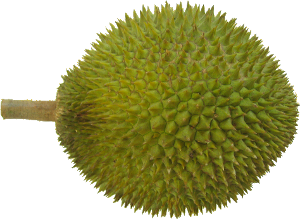
\includegraphics[height=1em]{../logos/logo-3-4-300.png}
}

\renewcommand{\headrulewidth}{.1pt}
\renewcommand{\footrulewidth}{0pt}

% \fancyfoot[c]{}
% \fancyfoot[R]{\footnotesize{\thepage}}



%%%%%%%%%%%%%%%%%%%%%%%%%%%%%%%%%%%%%%%%%%%%%%%%%%%%%%%%%%%%
% TIKZ
%%%%%%%%%%%%%%%%%%%%%%%%%%%%%%%%%%%%%%%%%%%%%%%%%%%%%%%%%%%%
\usepackage[svgnames,table]{xcolor}

\usepackage{pgf}
\usepackage{tikz}
\usetikzlibrary{arrows,automata,decorations.pathmorphing}
% Couleurs

\definecolor{darkblue}{rgb}{0.0,0.0,0.6}
\definecolor{darkgreen}{rgb}{0, 0.5, 0}
\definecolor{URLCOLOR}{rgb}{.4, .4, .7}


\definecolor{turquoise}{rgb}{0 0.41 0.41}
\definecolor{rouge}{rgb}{0.79 0.0 0.1}
\definecolor{vert}{rgb}{0.15 0.4 0.1}
\definecolor{mauve}{rgb}{0.6 0.4 0.8}
\definecolor{violet}{rgb}{0.58 0. 0.41}
\definecolor{orange}{rgb}{0.8 0.4 0.2}
\definecolor{bleu}{rgb}{0.39, 0.58, 0.93}
\definecolor{gris}{rgb}{0.6,0.6,0.6}
\definecolor{grisfonce}{rgb}{0.4,0.4,0.4}
% Jeu de couleurs pales
\definecolor{cpale1}{rgb}{1, 0.3, 0.3}
\definecolor{cpale2}{rgb}{0.3, 1, 0.3}
\definecolor{cpale3}{rgb}{0.3, 0.3, 1}
\definecolor{cpale4}{rgb}{1, 0.3, 1}
\definecolor{cpale5}{rgb}{1, 1, 0.3}
\definecolor{cpale6}{rgb}{0.3, 1, 1}
\definecolor{cpale7}{rgb}{0.9, 0.6, 0.2}
\definecolor{cpale8}{rgb}{0.7, 0.4, 1}
\definecolor{cpale9}{rgb}{0.5, 1, 0.75}
\definecolor{cpale10}{rgb}{0.8, 0.7, 0.6}
\definecolor{cpale11}{rgb}{0.6, 0.7, 0.8}
\definecolor{cpale12}{rgb}{0.2, 0.5, 0.9}
\definecolor{cpale13}{rgb}{0.5, 0.9, 0.2}
\definecolor{cpale14}{rgb}{0.9, 0.2, 0.5}
\definecolor{cpale15}{rgb}{0.7, 0.7, 0.7}
\definecolor{cpale16}{rgb}{0.8, 0.8, 0.5}


%%%%%%%%%%%%%%%%%%%%%%%%%%%%%%%%%%%%%%%%%%%%%%%%%%%%%%%%%%%%
% CLEVER REFERENCES
%%%%%%%%%%%%%%%%%%%%%%%%%%%%%%%%%%%%%%%%%%%%%%%%%%%%%%%%%%%%
\usepackage[capitalise,english,nameinlink]{cleveref} % load after algorithm2e and hyperref
% \crefname{line}{\text{line}}{\text{lines}} % to remove the capital


%%%%%%%%%%%%%%%%%%%%%%%%%%%%%%%%%%%%%%%%%%%%%%%%%%%%%%%%%%%%
% CONSTANTS
%%%%%%%%%%%%%%%%%%%%%%%%%%%%%%%%%%%%%%%%%%%%%%%%%%%%%%%%%%%%
%-%-%-%-%-%-%-%-%-%-%-%-%-%-%-%-%-%-%-%-%-%-%-%-%-%-%-%-%-%
% MATHS
%-%-%-%-%-%-%-%-%-%-%-%-%-%-%-%-%-%-%-%-%-%-%-%-%-%-%-%-%-%
% Variables
\def\init{\ensuremath{\textsf{init}}} % \xspace
\newcommand{\A}{\mathcal{A}}
\newcommand{\Action}{\ensuremath{\Sigma}}
\newcommand{\action}{a}
\newcommand{\ArithExpr}{\mathcal{AE}} % (#1)% set of all constraints over some set
\newcommand{\ArithExprD}{\ArithExpr(\DVar)}
\newcommand{\ArithExprR}{\ArithExpr(\RVar)}
\newcommand{\ArithExprI}{\ArithExpr(\IVar)}
\newcommand{\ArithExprB}{\ArithExpr(\BVar)}
\newcommand{\ArithExprW}{\ArithExpr(\WVar)}
% \newcommand{\ArithExprA}{\ArithExpr(\AVar)}
\newcommand{\C}{C}
\newcommand{\Cinit}{\C_\init} % initial constraint
\newcommand{\Clock}{X} % set of clocks
\newcommand{\ClockCard}{H} % cardinality of clocks
\newcommand{\clock}{x} % clock
\newcommand{\clockval}{w} % clock valuation
\newcommand{\Cupdates}{\Clock_\mathsf{up}}
\newcommand{\Dupdates}{\DVar_\mathsf{up}}
\newcommand{\dval}{\ensuremath{\delta}} % discrete variable
\newcommand{\DVar}{D} % set of discrete variables
\newcommand{\dvar}{d} % discrete variable
\newcommand{\DVarCard}{J} % cardinality of discrete variables
\newcommand{\rval}{\ensuremath{\rho}} % rational variable
\newcommand{\RVar}{R} % set of rational variables
\newcommand{\rvar}{r} % rational variable
\newcommand{\RVarCard}{J} % cardinality of rational variables
\newcommand{\ival}{\ensuremath{\i}} % integer variable
\newcommand{\IVar}{I} % set of integer variables
\newcommand{\ivar}{i} % integer variable
\newcommand{\IVarCard}{K} % cardinality of integer variables
\newcommand{\bval}{\ensuremath{\beta}} % boolean variable
\newcommand{\BVar}{B} % set of boolean variables
\newcommand{\bvar}{b} % boolean variable
\newcommand{\BVarCard}{L} % cardinality of boolean variables
% \newcommand{\wval}{\ensuremath{\omega}} % binary variable
\newcommand{\WVar}{W} % set of binary word variables
\newcommand{\wvar}{w} % binary word variable % TODO: conflict
% \newcommand{\WVarCard}{M} % cardinality of binary word variables  % TODO: conflict

% \newcommand{\aval}{\ensuremath{\alpha}} % array variable
% \newcommand{\AVar}{A} % set of array variables
% \newcommand{\ElVar}{El} % set of element of array variables
% \newcommand{\avar}{t} % array variable
% \newcommand{\AVarCard}{N} % cardinality of array variables

% \newcommand{\DVarinit}{\DVar_\init} % discrete variable
\newcommand{\edge}{e}
\newcommand{\flow}{\ensuremath{\mathit{flow}}}
\newcommand{\guard}{g}
\newcommand{\invariant}{I}
\newcommand{\LConstraint}{\mathcal{LC}} % (#1)% set of all constraints over some set
\newcommand{\LConstraintD}{\LConstraint(\RVar)}
\newcommand{\LConstraintXP}{\LConstraint(\Clock \cup \Param)}
\newcommand{\LConstraintXPD}{\LConstraint(\Clock \cup \Param \cup \RVar)}
\newcommand{\lterm}{\mathit{lt}}
\newcommand{\LTerm}{\mathcal{LT}} % (#1)% set of all linear terms over some set
\newcommand{\LTermR}{\LTerm(\RVar)}
\newcommand{\LTermXPD}{\LTerm(\Clock \cup \Param \cup \RVar)}
\newcommand{\loc}{\ell} % location
\newcommand{\locinit}{\loc_\init}
\newcommand{\Loc}{L} % set of locations
\newcommand{\Param}{P} % set of parameters
\newcommand{\param}{p} % parameter
\newcommand{\ParamCard}{M} % number of parameters
\newcommand{\pval}{v} % parameter valuation
% \newcommand{\resets}{R}
\newcommand{\steps}{ {\rightarrow} }
% \newcommand{\stopwatches}{\mathit{SW}}
\newcommand{\tuple}[1]{\langle#1\rangle}
\newcommand{\unobs}{\ensuremath{\epsilon}}
\newcommand{\Var}{\mathit{Var}} % set of variables
\newcommand{\var}{\mathit{z}} % variable
\newcommand{\VarCard}{N} % cardinality of variables % TODO: conflict

% Sets
\newcommand{\setA}{\ensuremath{\mathbb A}}
\newcommand{\setB}{\ensuremath{\mathbb B}}
% \newcommand{\setW}{\ensuremath{\mathbb W}}
\newcommand{\setN}{\ensuremath{\mathbb N}}
\newcommand{\setQ}{\ensuremath{\mathbb Q}}
\newcommand{\setQplus}{\ensuremath{\mathbb Q}_{\geq 0}}
\newcommand{\setR}{\ensuremath{\mathbb R}}
\newcommand{\setRplus}{\ensuremath{\setR_{\geq 0}}}
\newcommand{\setZ}{\ensuremath{\mathbb Z}}

\newcommand{\BFalse}{\ensuremath{\mathbf{false}}}
\newcommand{\BTrue}{\ensuremath{\mathbf{true}}}

% Units
\newcommand{\micros}{\mathit{\mu s}}
\newcommand{\nanos}{ns}

% Noms
\newcommand{\pio}{\pi_0}

% Symbols
\newcommand{\emptystring}{\ensuremath{\epsilon}}
\newcommand{\fleche}[1]{\stackrel{#1}{\rightarrow}}
\newcommand{\Fleche}[1]{\stackrel{#1}{\Rightarrow}}
% \newcommand{\steps}[0]{ {\rightarrow} }


%-%-%-%-%-%-%-%-%-%-%-%-%-%-%-%-%-%-%-%-%-%-%-%-%-%-%-%-%-%
% ALGORITHMES
%-%-%-%-%-%-%-%-%-%-%-%-%-%-%-%-%-%-%-%-%-%-%-%-%-%-%-%-%-%
% Algorithmes PTA
\newcommand{\BC}{\ensuremath{\mathsf{BC}}}
\newcommand{\EFsynth}{\ensuremath{\mathsf{EFsynth}}}
\newcommand{\IM}{\ensuremath{\mathsf{IM}}}
\newcommand{\PDFC}{\ensuremath{\mathsf{PDFC}}}
\newcommand{\PRP}{\ensuremath{\mathsf{PRP}}}
\newcommand{\PRPC}{\ensuremath{\mathsf{PRPC}}}


%-%-%-%-%-%-%-%-%-%-%-%-%-%-%-%-%-%-%-%-%-%-%-%-%-%-%-%-%-%
% CONSTANTES DE CHAINES
%-%-%-%-%-%-%-%-%-%-%-%-%-%-%-%-%-%-%-%-%-%-%-%-%-%-%-%-%-%

% Outils
% \newcommand{\apron}{\textsc{Apron}}
\newcommand{\CosyVerif}{\emph{CosyVerif}}
\newcommand{\gdot}{\texttt{dot}}
\newcommand{\graphviz}{Graphviz}
\newcommand{\hytech}{{\sc HyTech}}
\newcommand{\imitator}{\textsf{IMITATOR}}
\newcommand{\imitatorExec}{\code{imitator}}
\newcommand{\IPTA}{IPTA}
\newcommand{\NIPTA}{NIPTA}
\newcommand{\ocaml}{OCaml}
\newcommand{\pat}{PAT}
\newcommand{\phaver}{PHAVer}
\newcommand{\phaverLite}{PHAVerLite}
% \newcommand{\polka}{NewPolka}
% \newcommand{\prism}{\textsc{Prism}}
% \newcommand{\red}{RED}
\newcommand{\uppaal}{\textsc{Uppaal}}
% \newcommand{\jani}{\textsc{The Jani Specification}}
\newcommand{\jani}{\textsc{Jani}}

\newcommand{\binimitator}{./imitator}


% Current version
\newcommand{\imitatorversion}{3.4-beta}
\newcommand{\imitatorversionname}{Cheese Durian}


%%%%%%%%%%%%%%%%%%%%%%%%%%%%%%%%%%%%%%%%%%%%%%%%%%%%%%%%%%%%
% THEOREMS
%%%%%%%%%%%%%%%%%%%%%%%%%%%%%%%%%%%%%%%%%%%%%%%%%%%%%%%%%%%%
\usepackage[framemethod=TikZ]{mdframed}

%------------------------------------------------------------
\theoremstyle{plain}
%------------------------------------------------------------


%------------------------------------------------------------
\theoremstyle{definition}
%------------------------------------------------------------
\newtheorem{mydefinition}{Definition}[chapter]
\newenvironment{definition}%
	{\begin{mdframed}[roundcorner=3pt,backgroundcolor=blue!7,linecolor=blue!70,linewidth=2]\begin{mydefinition}}
	{\end{mydefinition}\end{mdframed}}

\newtheorem{myexample}{Example}[chapter]
\newenvironment{example}
	{\begin{mdframed}[roundcorner=3pt,backgroundcolor=green!7,linecolor=green!70,linewidth=2]\begin{myexample}}
	{\end{myexample}\end{mdframed}}

%------------------------------------------------------------
\theoremstyle{remark}
%------------------------------------------------------------
\newtheorem{myremark}{Remark}[chapter]
\newenvironment{remark}
	{\begin{mdframed}[roundcorner=3pt,backgroundcolor=pink!7,linecolor=pink!70,linewidth=2]\begin{myremark}}
	{\end{myremark}\end{mdframed}}

\newtheorem{myhint}{Hint}[chapter]
\newenvironment{hint}
	{\begin{mdframed}[roundcorner=3pt,backgroundcolor=green!7,linecolor=green!70!black,linewidth=2]\begin{myhint}}
	{\end{myhint}\end{mdframed}}

\newtheorem{mywarning}{Warning} %[chapter]
\newenvironment{becareful}
	{\begin{mdframed}[roundcorner=3pt,backgroundcolor=red!20,linecolor=red!50!black,linewidth=2]\begin{mywarning}}
	{\end{mywarning}\end{mdframed}}

\newtheorem{myalias}{Syntax freedom} %[chapter]
\newenvironment{syntaxalias}
	{\begin{mdframed}[roundcorner=3pt,backgroundcolor=green!20,linecolor=green!50!black,linewidth=2]\begin{myalias}\small}
	{\end{myalias}\end{mdframed}}



%%%%%%%%%%%%%%%%%%%%%%%%%%%%%%%%%%%%%%%%%%%%%%%%%%%%%%%%%%%%
% FORMATING
%%%%%%%%%%%%%%%%%%%%%%%%%%%%%%%%%%%%%%%%%%%%%%%%%%%%%%%%%%%%

\hyphenation{IMITATOR}
\hyphenation{Uppaal}

% \newcommand{\paragraphe}[1]{\paragraph{#1.}}

% Non terminal in a grammar
\newcommand{\nt}[1]{$\langle$\emph{#1}$\rangle$}
% Rule name in a grammar
\newcommand{\regleGrammaire}[1]{\bigskip \noindent \nt{#1} :: \\}
% Not taken into account in the grammar
% \newcommand{\npec}[1]{\textcolor{green!50!black}{#1}}
\newcommand{\commentgrammar}[1]{\textcolor{black!50}{\texttt{/* #1 */}}}

\newcommand{\probleme}[2]{
	\medskip
	\noindent
	\fbox{
		\begin{minipage}{0.95\textwidth}
		\textbf{#1}

		#2
		\end{minipage}
	}

	\medskip
}

% \newcommand{\warningbox}[2]{
% 	\medskip
% 	\noindent
% 	\fcolorbox{red!50!black}{red!20}{
% 		\begin{minipage}{0.95\textwidth}
% 		\textbf{Warning: #1}
%
% 		#2
% 		\end{minipage}
% 	}
%
% 	\medskip
% }

% \newcommand{\commentaire}[1]{\textcolor{red}{\textbf{$\Leftarrow$  #1 $\Rightarrow$}}} % commentaire dans un paragraphe
% \newcommand{\commentaire}[1]{}


% Code integre au texte
% \newcommand{\code}[1]{\textbf{\texttt{#1}}}


\definecolor{imicolor}{rgb}{0, .4, .4}
\newcommand{\styleIMI}[1]{\textcolor{imicolor}{\texttt{#1}}}

\definecolor{optioncolor}{rgb}{.4, 0, .4}
\newcommand{\styleOption}[1]{\textcolor{optioncolor}{\texttt{#1}}}
\newcommand{\styleOptionValue}[1]{\textcolor{optioncolor}{\texttt{#1}}}

\definecolor{pathcolor}{rgb}{1, .5, 0}
\newcommand{\stylePath}[1]{\textcolor{pathcolor}{\texttt{#1}}}

\definecolor{filecontentcolor}{rgb}{.1, .4, .2}
\newcommand{\styleFileContent}[1]{\textcolor{filecontentcolor}{\texttt{#1}}}

\newcommand{\GitHubIMI}{\href{https://github.com/imitator-model-checker/imitator}{GitHub}}

% \newcommand{\styleCommand}[1]{
% 	\medskip
% 
% 	% \mbox{}\hspace{.5cm}
% 	\noindent\fcolorbox{white}{black!90}{
% 		\textcolor{yellow!30}{\$\ \ \texttt{#1}}
% 	}
% 
% 	\medskip
% 
% }

% \newcommand{\styleTerminalOutput}[1]{
% 	\medskip
% 
% 	% \mbox{}\hspace{.5cm}
% 	\noindent\fcolorbox{white}{black!90}{
% 	\begin{minipage}{.97\textwidth}
% 		\textcolor{yellow!30}{\texttt{#1}}
% 	\end{minipage}
% 	}
% 
% 	\medskip
% 
% }


%%%%%%%%%%%%%%%%%%%%%%%%%%%%%%%%%%%%%%%%%%%%%%%%%%%%%%%%%%%%
% COLORS AND TABLES
%%%%%%%%%%%%%%%%%%%%%%%%%%%%%%%%%%%%%%%%%%%%%%%%%%%%%%%%%%%%
\newcommand{\cellHeader}[1]{\cellcolor{blue!20}\textbf{#1}}
\newcommand{\rowHeader}{\rowcolor{blue!20}}

\definecolor{vertfonce}{rgb}{0.0, 0.5, 0.0}
\definecolor{rougefonce}{rgb}{1, 0.0, 0.0}
\newcommand{\compyes}{$\textcolor{vertfonce}{\mathbf{\surd}}$}
\newcommand{\compno}{$\textcolor{rougefonce}{\mathbf{\times}}$}

\newcommand{\cellYes}{\cellcolor{green!20}\textbf{\compyes}}
\newcommand{\cellYesNo}{\cellcolor{orange!20}\textbf{\compyes/\compno}}
\newcommand{\cellNo}{\cellcolor{red!20}\textbf{\compno}}
\newcommand{\cellNA}{\cellcolor{black!20}N/A}
\newcommand{\cellUnclear}{\cellcolor{yellow!20}\textbf{?}}

%%%%%%%%%%%%%%%%%%%%%%%%%%%%%%%%%%%%%%%%%%%%%%%%%%%%%%%%%%%%
% I.E. / E.G. / W.R.T.
%%%%%%%%%%%%%%%%%%%%%%%%%%%%%%%%%%%%%%%%%%%%%%%%%%%%%%%%%%%%

% Helps to spot the places where macros are NOT used
\ifdefined \DraftVersion
 	\definecolor{colorok}{RGB}{80,80,150}
\else
	\definecolor{colorok}{RGB}{0,0,0}
\fi

% \newcommand{\eg}{\textcolor{colorok}{\textit{e.g.}}\xspace}
% \newcommand{\ie}{\textcolor{colorok}{\textit{i.e.}}\xspace}
% \newcommand{\wrt}{\textcolor{colorok}{w.r.t.}\xspace}
\newcommand{\adhoc}{\textcolor{colorok}{\textit{ad-hoc}\@}}
\newcommand{\eg}{\textcolor{colorok}{\textit{e.g.},\@}}
\newcommand{\ie}{\textcolor{colorok}{\textit{i.e.},\@}}
\newcommand{\wrt}{\textcolor{colorok}{w.r.t.}\@}





%%%%%%%%%%%%%%%%%%%%%%%%%%%%%%%%%%%%%%%%%%%%%%%%%%%%%%%%%%%%
% IMITATOR FILES
%%%%%%%%%%%%%%%%%%%%%%%%%%%%%%%%%%%%%%%%%%%%%%%%%%%%%%%%%%%%
\definecolor{bggcolor}{rgb}{0.95,0.95,0.95}
\definecolor{commentscolor}{rgb}{0.5,0.5,0.6}
% \definecolor{numberscolor}{rgb}{0.1,.5,0.1}
\definecolor{keywordscolor}{rgb}{0.0, 0.0, 1.0}
\definecolor{numberscolor}{rgb}{0.6, 0.6, 0.6}
% \definecolor{stringscolor}{rgb}{1,0.6,0.6}
\definecolor{binarycolor}{rgb}{1, 0.0, 0.0}


\usepackage{listings}
\newcommand{\IncludeIMIfile}[1]{
	\lstset{style=IMITATORmodel}
	\lstinputlisting[
		basicstyle=\footnotesize,
% 		breaklines=true,
% 		breakatwhitespace=true,
		columns=fixed,
% 		numbers=left,
% 		frame=single,
% 		numberstyle=\tiny,
% 		tabsize=4,
% 		title=\lstname
	]{#1}
}

\newcommand{\IncludeIMIproperty}[1]{
	\lstset{style=IMITATORproperty}
	\lstinputlisting[]{#1}
}

\lstdefinestyle{IMITATORmodel}{
	backgroundcolor=\color{white},   % choose the background color; you must add \usepackage{color} or \usepackage{xcolor}; should come as last argument
	basicstyle=\tt\footnotesize,        % the size of the fonts that are used for the code
	breakatwhitespace=true,         % sets if automatic breaks should only happen at whitespace
	breaklines=true,                 % sets automatic line breaking
	%   captionpos=b,                    % sets the caption-position to bottom
	commentstyle=\color{commentscolor},    % comment style
	escapeinside={\%*}{*)},          % if you want to add LaTeX within your code
	extendedchars=true,              % lets you use non-ASCII characters; for 8-bits encodings only, does not work with UTF-8
	%   firstnumber=1,                % start line enumeration with line 1000
	frame=single,	                   % adds a frame around the code
	keepspaces=true,                 % keeps spaces in text, useful for keeping indentation of code (possibly needs columns=flexible)
	keywordstyle=\bfseries\color{keywordscolor},       % keyword style
	language=caml,                 % the language of the code
	deletekeywords={done},            % if you want to delete keywords from the given language; WARNING! must be set AFTER the `language=…`
	morekeywords={
		accepting, and, array, automaton, binary, bool, clock, constant, continuous, discrete, do, seq, end, False, fill_left, fill_right, flow, forward, from, goto, if, in, init, int, initially, invariant, loc, logand, lognot, logor, logxor, not, or, parameter, projectresult, rational, rat, shift_left, shift_right, stop, sync, sync, synclabs, True, urgent, var, when, while, fn
	},
	numbers=right,                    % where to put the line-numbers; possible values are (none, left, right)
	numbersep=5pt,                   % how far the line-numbers are from the code
	numberstyle=\tiny\color{numberscolor}, % the style that is used for the line-numbers
	rulecolor=\color{black},         % if not set, the frame-color may be changed on line-breaks within not-black text (e.g. comments (green here))
	showspaces=false,                % show spaces everywhere adding particular underscores; it overrides 'showstringspaces'
	showstringspaces=false,          % underline spaces within strings only
	showtabs=false,                  % show tabs within strings adding particular underscores
	stepnumber=1,                    % the step between two line-numbers. If it's 1, each line will be numbered
% 	stringstyle=\color{stringscolor},     % string literal style
	tabsize=2,	                   % sets default tabsize to 2 spaces
	sensitive=false,
% 	morecomment=[l][\color{gray}]{--},
% 	morecomment=[s][keywordstyle]{"}{"},
% 	morecomment=[s]{/*}{*/},
% 	morestring=[s][\color{red}]{0b}, % values: b,d,m,s(*2?)
	moredelim=[s][\color{binarycolor}]{0b}{\ },
	moredelim=[s][\color{red}]{\#}{\ },
	morecomment=[s][\color{commentscolor}]{(*}{*)},
		% values: lfdnms
	% For UTF-8
	inputencoding=utf8,
    extendedchars=true,
    literate=
        {á}{{\'a}}1  {é}{{\'e}}1  {í}{{\'i}}1 {ó}{{\'o}}1  {ú}{{\'u}}1
      {Á}{{\'A}}1  {É}{{\'E}}1  {Í}{{\'I}}1 {Ó}{{\'O}}1  {Ú}{{\'U}}1
      {à}{{\`a}}1  {è}{{\`e}}1  {ì}{{\`i}}1 {ò}{{\`o}}1  {ù}{{\`u}}1
      {À}{{\`A}}1  {È}{{\'E}}1  {Ì}{{\`I}}1 {Ò}{{\`O}}1  {Ù}{{\`U}}1
      {ä}{{\"a}}1  {ë}{{\"e}}1  {ï}{{\"i}}1 {ö}{{\"o}}1  {ü}{{\"u}}1
      {Ä}{{\"A}}1  {Ë}{{\"E}}1  {Ï}{{\"I}}1 {Ö}{{\"O}}1  {Ü}{{\"U}}1
      {â}{{\^a}}1  {ê}{{\^e}}1  {î}{{\^i}}1 {ô}{{\^o}}1  {û}{{\^u}}1
      {Â}{{\^A}}1  {Ê}{{\^E}}1  {Î}{{\^I}}1 {Ô}{{\^O}}1  {Û}{{\^U}}1
      {œ}{{\oe}}1  {Œ}{{\OE}}1  {æ}{{\ae}}1 {Æ}{{\AE}}1  {ß}{{\ss}}1
      {ç}{{\c c}}1 {Ç}{{\c C}}1 {ø}{{\o}}1  {Ø}{{\O}}1   {å}{{\r a}}1
      {Å}{{\r A}}1 {ã}{{\~a}}1  {õ}{{\~o}}1 {Ã}{{\~A}}1  {Õ}{{\~O}}1
      {ñ}{{\~n}}1  {Ñ}{{\~N}}1  {¿}{{?`}}1  {¡}{{!`}}1
      {ā}{{\=a}}1  {Ā}{{\=A}}1 {ē}{{\=e}}1  {Ē}{{\=E}}1 {ī}{{\=i}}1 {Ī}{{\=I}}1 {ō}{{\=o}}1 {Ō}{{\=O}}1 {ū}{{\=u}}1 {Ū}{{\=U}}1 
      ,
}



\lstdefinestyle{IMITATORproperty}{
  backgroundcolor=\color{bggcolor},   % choose the background color; you must add \usepackage{color} or \usepackage{xcolor}; should come as last argument
  basicstyle=\tt\scriptsize,        % the size of the fonts that are used for the code
%   breakatwhitespace=false,         % sets if automatic breaks should only happen at whitespace
  breaklines=true,                 % sets automatic line breaking
%   captionpos=b,                    % sets the caption-position to bottom
  commentstyle=\color{commentscolor},    % comment style
%   deletekeywords={},            % if you want to delete keywords from the given language
  escapeinside={\%*}{*)},          % if you want to add LaTeX within your code
  extendedchars=true,              % lets you use non-ASCII characters; for 8-bits encodings only, does not work with UTF-8
%   firstnumber=1000,                % start line enumeration with line 1000
  frame=single,	                   % adds a frame around the code
  keepspaces=true,                 % keeps spaces in text, useful for keeping indentation of code (possibly needs columns=flexible)
  keywordstyle=\bfseries\color{keywordscolor},       % keyword style
%   language=caml,                 % the language of the code
  morekeywords={accepting, AGnot, always, BCcover, BCrandom, BCshuffle, before, Cycle, CycleThrough, DeadlockFree, EF, EFpmin, EFpmax, EFtmin, everytime, eventually, happened, has, IM, loc, next, once, pattern, PRP, PRPC, property,sequence,synth,within,witness},            % if you want to add more keywords to the set
  numbers=none,                    % where to put the line-numbers; possible values are (none, left, right)
%   numbersep=5pt,                   % how far the line-numbers are from the code
%   numberstyle=\tiny\color{bggcolor}, % the style that is used for the line-numbers
%   rulecolor=\color{black},         % if not set, the frame-color may be changed on line-breaks within not-black text (e.g. comments (green here))
%   showspaces=false,                % show spaces everywhere adding particular underscores; it overrides 'showstringspaces'
%   showstringspaces=false,          % underline spaces within strings only
%   showtabs=false,                  % show tabs within strings adding particular underscores
%   stepnumber=2,                    % the step between two line-numbers. If it's 1, each line will be numbered
%   stringstyle=\color{stringscolor},     % string literal style
%   tabsize=2,	                   % sets default tabsize to 2 spaces
%   title=\lstname                   % show the filename of files included with \lstinputlisting; also try caption instead of title
	morecomment=[s][\color{commentscolor}]{(*}{*)},
	% For UTF-8
	inputencoding=utf8,
    extendedchars=true,
    literate=
        {á}{{\'a}}1  {é}{{\'e}}1  {í}{{\'i}}1 {ó}{{\'o}}1  {ú}{{\'u}}1
      {Á}{{\'A}}1  {É}{{\'E}}1  {Í}{{\'I}}1 {Ó}{{\'O}}1  {Ú}{{\'U}}1
      {à}{{\`a}}1  {è}{{\`e}}1  {ì}{{\`i}}1 {ò}{{\`o}}1  {ù}{{\`u}}1
      {À}{{\`A}}1  {È}{{\'E}}1  {Ì}{{\`I}}1 {Ò}{{\`O}}1  {Ù}{{\`U}}1
      {ä}{{\"a}}1  {ë}{{\"e}}1  {ï}{{\"i}}1 {ö}{{\"o}}1  {ü}{{\"u}}1
      {Ä}{{\"A}}1  {Ë}{{\"E}}1  {Ï}{{\"I}}1 {Ö}{{\"O}}1  {Ü}{{\"U}}1
      {â}{{\^a}}1  {ê}{{\^e}}1  {î}{{\^i}}1 {ô}{{\^o}}1  {û}{{\^u}}1
      {Â}{{\^A}}1  {Ê}{{\^E}}1  {Î}{{\^I}}1 {Ô}{{\^O}}1  {Û}{{\^U}}1
      {œ}{{\oe}}1  {Œ}{{\OE}}1  {æ}{{\ae}}1 {Æ}{{\AE}}1  {ß}{{\ss}}1
      {ç}{{\c c}}1 {Ç}{{\c C}}1 {ø}{{\o}}1  {Ø}{{\O}}1   {å}{{\r a}}1
      {Å}{{\r A}}1 {ã}{{\~a}}1  {õ}{{\~o}}1 {Ã}{{\~A}}1  {Õ}{{\~O}}1
      {ñ}{{\~n}}1  {Ñ}{{\~N}}1  {¿}{{?`}}1  {¡}{{!`}}1
      {ā}{{\=a}}1  {Ā}{{\=A}}1 {ē}{{\=e}}1  {Ē}{{\=E}}1 {ī}{{\=i}}1 {Ī}{{\=I}}1 {ō}{{\=o}}1 {Ō}{{\=O}}1 {ū}{{\=u}}1 {Ū}{{\=U}}1 
      ,
}


\definecolor{commentscolorterminal}{rgb}{0.6,0.6,0.6}
% \definecolor{numberscolorterminal}{rgb}{0.3,.3,0.3}
\definecolor{stringscolorterminal}{rgb}{.6,1,0.6}

\lstdefinestyle{terminal}{
	backgroundcolor=\color{black},   % choose the background color; you must add \usepackage{color} or \usepackage{xcolor}; should come as last argument
	basicstyle=\ttfamily\small\color{yellow},        % the size of the fonts that are used for the code
	breakatwhitespace=true,         % sets if automatic breaks should only happen at whitespace
	breaklines=true,                 % sets automatic line breaking
	%   captionpos=b,                    % sets the caption-position to bottom
	commentstyle=\color{commentscolorterminal},    % comment style
	escapeinside={\%*}{*)},          % if you want to add LaTeX within your code
	%   firstnumber=1,                % start line enumeration with line 1000
	frame=single,	                   % adds a frame around the code
	keepspaces=true,                 % keeps spaces in text, useful for keeping indentation of code (possibly needs columns=flexible)
	keywordstyle=\bfseries\color{orange},       % keyword style
	language=bash,                 % the language of the code
% 	deletekeywords={done},            % if you want to delete keywords from the given language; WARNING! must be set AFTER the `language=…`
	morekeywords={
		grep, imitator
	},
	numbers=none,                    % where to put the line-numbers; possible values are (none, left, right)
% 	numbersep=5pt,                   % how far the line-numbers are from the code
% 	numberstyle=\tiny\color{numberscolorterminal}, % the style that is used for the line-numbers
	rulecolor=\color{black},         % if not set, the frame-color may be changed on line-breaks within not-black text (e.g. comments (green here))
	showspaces=false,                % show spaces everywhere adding particular underscores; it overrides 'showstringspaces'
	showstringspaces=false,          % underline spaces within strings only
	showtabs=false,                  % show tabs within strings adding particular underscores
	stepnumber=1,                    % the step between two line-numbers. If it's 1, each line will be numbered
	stringstyle=\color{stringscolorterminal},     % string literal style
	tabsize=2,	                   % sets default tabsize to 2 spaces
	sensitive=false,
	% For UTF-8
	inputencoding=utf8,
    extendedchars=true,
    literate=
        {á}{{\'a}}1  {é}{{\'e}}1  {í}{{\'i}}1 {ó}{{\'o}}1  {ú}{{\'u}}1
      {Á}{{\'A}}1  {É}{{\'E}}1  {Í}{{\'I}}1 {Ó}{{\'O}}1  {Ú}{{\'U}}1
      {à}{{\`a}}1  {è}{{\`e}}1  {ì}{{\`i}}1 {ò}{{\`o}}1  {ù}{{\`u}}1
      {À}{{\`A}}1  {È}{{\'E}}1  {Ì}{{\`I}}1 {Ò}{{\`O}}1  {Ù}{{\`U}}1
      {ä}{{\"a}}1  {ë}{{\"e}}1  {ï}{{\"i}}1 {ö}{{\"o}}1  {ü}{{\"u}}1
      {Ä}{{\"A}}1  {Ë}{{\"E}}1  {Ï}{{\"I}}1 {Ö}{{\"O}}1  {Ü}{{\"U}}1
      {â}{{\^a}}1  {ê}{{\^e}}1  {î}{{\^i}}1 {ô}{{\^o}}1  {û}{{\^u}}1
      {Â}{{\^A}}1  {Ê}{{\^E}}1  {Î}{{\^I}}1 {Ô}{{\^O}}1  {Û}{{\^U}}1
      {œ}{{\oe}}1  {Œ}{{\OE}}1  {æ}{{\ae}}1 {Æ}{{\AE}}1  {ß}{{\ss}}1
      {ç}{{\c c}}1 {Ç}{{\c C}}1 {ø}{{\o}}1  {Ø}{{\O}}1   {å}{{\r a}}1
      {Å}{{\r A}}1 {ã}{{\~a}}1  {õ}{{\~o}}1 {Ã}{{\~A}}1  {Õ}{{\~O}}1
      {ñ}{{\~n}}1  {Ñ}{{\~N}}1  {¿}{{?`}}1  {¡}{{!`}}1
      {ā}{{\=a}}1  {Ā}{{\=A}}1 {ē}{{\=e}}1  {Ē}{{\=E}}1 {ī}{{\=i}}1 {Ī}{{\=I}}1 {ō}{{\=o}}1 {Ō}{{\=O}}1 {ū}{{\=u}}1 {Ū}{{\=U}}1 
    ,
}

% Define empty language
\lstdefinelanguage{none}{
  identifierstyle=
}

\lstdefinestyle{terminaloutput}{
	backgroundcolor=\color{black},   % choose the background color; you must add \usepackage{color} or \usepackage{xcolor}; should come as last argument
	basicstyle=\ttfamily\small\color{yellow},        % the size of the fonts that are used for the code
	breakatwhitespace=true,         % sets if automatic breaks should only happen at whitespace
	breaklines=true,                 % sets automatic line breaking
	%   captionpos=b,                    % sets the caption-position to bottom
	commentstyle=\color{commentscolorterminal},    % comment style
	escapeinside={\%*}{*)},          % if you want to add LaTeX within your code
	extendedchars=true,              % lets you use non-ASCII characters; for 8-bits encodings only, does not work with UTF-8
	%   firstnumber=1,                % start line enumeration with line 1000
	frame=single,	                   % adds a frame around the code
	keepspaces=true,                 % keeps spaces in text, useful for keeping indentation of code (possibly needs columns=flexible)
% 	keywordstyle=\bfseries\color{orange},       % keyword style
	language=none,                 % the language of the code
% 	deletekeywords={done},            % if you want to delete keywords from the given language; WARNING! must be set AFTER the `language=…`
% 	morekeywords={
% 		imitator
% 	},
	numbers=none,                    % where to put the line-numbers; possible values are (none, left, right)
% 	numbersep=5pt,                   % how far the line-numbers are from the code
% 	numberstyle=\tiny\color{numberscolorterminal}, % the style that is used for the line-numbers
	rulecolor=\color{black},         % if not set, the frame-color may be changed on line-breaks within not-black text (e.g. comments (green here))
	showspaces=false,                % show spaces everywhere adding particular underscores; it overrides 'showstringspaces'
	showstringspaces=false,          % underline spaces within strings only
	showtabs=false,                  % show tabs within strings adding particular underscores
	stepnumber=1,                    % the step between two line-numbers. If it's 1, each line will be numbered
	stringstyle=\color{stringscolorterminal},     % string literal style
	tabsize=2,	                   % sets default tabsize to 2 spaces
	sensitive=false,
	% For UTF-8
	inputencoding=utf8,
    extendedchars=true,
    literate=
        {á}{{\'a}}1  {é}{{\'e}}1  {í}{{\'i}}1 {ó}{{\'o}}1  {ú}{{\'u}}1
      {Á}{{\'A}}1  {É}{{\'E}}1  {Í}{{\'I}}1 {Ó}{{\'O}}1  {Ú}{{\'U}}1
      {à}{{\`a}}1  {è}{{\`e}}1  {ì}{{\`i}}1 {ò}{{\`o}}1  {ù}{{\`u}}1
      {À}{{\`A}}1  {È}{{\'E}}1  {Ì}{{\`I}}1 {Ò}{{\`O}}1  {Ù}{{\`U}}1
      {ä}{{\"a}}1  {ë}{{\"e}}1  {ï}{{\"i}}1 {ö}{{\"o}}1  {ü}{{\"u}}1
      {Ä}{{\"A}}1  {Ë}{{\"E}}1  {Ï}{{\"I}}1 {Ö}{{\"O}}1  {Ü}{{\"U}}1
      {â}{{\^a}}1  {ê}{{\^e}}1  {î}{{\^i}}1 {ô}{{\^o}}1  {û}{{\^u}}1
      {Â}{{\^A}}1  {Ê}{{\^E}}1  {Î}{{\^I}}1 {Ô}{{\^O}}1  {Û}{{\^U}}1
      {œ}{{\oe}}1  {Œ}{{\OE}}1  {æ}{{\ae}}1 {Æ}{{\AE}}1  {ß}{{\ss}}1
      {ç}{{\c c}}1 {Ç}{{\c C}}1 {ø}{{\o}}1  {Ø}{{\O}}1   {å}{{\r a}}1
      {Å}{{\r A}}1 {ã}{{\~a}}1  {õ}{{\~o}}1 {Ã}{{\~A}}1  {Õ}{{\~O}}1
      {ñ}{{\~n}}1  {Ñ}{{\~N}}1  {¿}{{?`}}1  {¡}{{!`}}1
      {ā}{{\=a}}1  {Ā}{{\=A}}1 {ē}{{\=e}}1  {Ē}{{\=E}}1 {ī}{{\=i}}1 {Ī}{{\=I}}1 {ō}{{\=o}}1 {Ō}{{\=O}}1 {ū}{{\=u}}1 {Ū}{{\=U}}1 
      ,
}

\lstnewenvironment{terminal}[0]
	{%
		\lstset{style=terminal}
	}%
	{}

\lstnewenvironment{terminaloutput}[0]
	{%
		\lstset{style=terminaloutput}
	}%
	{}

\lstnewenvironment{IMITATORmodel}[0]
	{%
		\lstset{style=IMITATORmodel}
	}%
	{}

\lstnewenvironment{IMITATORproperty}[0]
	{%
		\lstset{style=IMITATORproperty}
	}%
	{}


%%%%%%%%%%%%%%%%%%%%%%%%%%%%%%%%%%%%%%%%%%%%%%%%%%%%%%%%%%%%
% bibLaTeX
%%%%%%%%%%%%%%%%%%%%%%%%%%%%%%%%%%%%%%%%%%%%%%%%%%%%%%%%%%%%
\usepackage[backend=biber,backref=true,style=alphabetic,url=false,doi=true,defernumbers=true,sorting=anyt,maxnames=99]{biblatex} % tlmgr install biblatex etoolbox logreq
\addbibresource{biblio.bib}

% Reformat DOI
\renewbibmacro*{doi+eprint+url}{%
	\iftoggle{bbx:doi}
		{\color{black!40}\footnotesize\printfield{doi}}
		{}%
	\newunit\newblock
	\iftoggle{bbx:eprint}
		{\usebibmacro{eprint}}
		{}%
	\newunit\newblock
	\iftoggle{bbx:url}
% 		{\color{black!40}\footnotesize\printfield{url}}
		{\usebibmacro{url+urldate}}
		{}%
}


%%%%%%%%%%%%%%%%%%%%%%%%%%%%%%%%%%%%%%%%%%%%%%%%%%%%%%%%%%%%
% MISC
%%%%%%%%%%%%%%%%%%%%%%%%%%%%%%%%%%%%%%%%%%%%%%%%%%%%%%%%%%%%

\sloppy
